% JarvisTEC - project report.
% Overleaf: upload main.tex and the figures/ folder, compile with pdfLaTeX.
\documentclass[11pt,letterpaper]{article}
\usepackage[utf8]{inputenc}
\usepackage[T1]{fontenc}
\usepackage[english]{babel}
\usepackage[margin=2.5cm]{geometry}
\usepackage{booktabs}
\usepackage{tabularx}
\usepackage{graphicx}
\usepackage{float}
\usepackage{xcolor}
\usepackage{enumitem}
\usepackage[hidelinks]{hyperref}

\newcommand{\code}[1]{\texttt{#1}}
\graphicspath{{figures/}}

\begin{document}

% ------------------------------------------------------------- Cover page
\begin{titlepage}
\centering
{\large Instituto Tecnológico de Costa Rica\par}
{\large San Carlos Local Technological Campus\par}
{\large School of Computer Engineering\par}
\vspace{2.5cm}
{\large IC-6200 Artificial Intelligence\par}
\vspace{1.5cm}
{\Huge\bfseries JarvisTEC\par}
\vspace{0.4cm}
{\Large A voice and vision personal assistant that runs machine learning models\par}
\vspace{2.5cm}
{\large Group project\par}
\vspace{1.5cm}
{\large Team members:\par}
Anthony Jafeth Arias Robleto --- 2020007243\par
Randy Espinoza Downing --- 2021031263\par
Kenneth Jhoan Araya Arguedas --- 2024177221\par
\vspace{1.5cm}
{\large Professor: Ing. Efrén Jiménez Delgado\par}
\vfill
{\large First semester, 2026\par}
\end{titlepage}

\tableofcontents
\newpage

% ------------------------------------------------------ Proposed solution
\section{Proposed solution}

JarvisTEC is a personal assistant that takes instructions by voice or text, watches the user's face through the camera and answers by running a machine learning model. The user says, for example, ``JarvisTEC, wine quality''; the system turns the speech into text, identifies which of the ten models the instruction refers to, runs the model and answers with a sentence, which is also read aloud. When the camera is on, the system estimates the user's dominant emotion and adapts the tone of the answer and the color of the interface. The interface, the commands and the answers are in English.

\subsection{Components}

\begin{description}[leftmargin=0.5cm]
\item[Web interface.] A page written in HTML, CSS and JavaScript with no dependencies, styled as a reactor after the reference interface of the assignment. It captures camera frames (WebRTC), listens to the microphone, animates the reactor with the real microphone volume and reads the answer with the browser's speech synthesis. It lists the available commands and, for each model, shows a form generated automatically from the model's inputs, so the user can query the model with their own values.
\item[REST API.] A FastAPI service that exposes every resource of the system (Table~\ref{tab:api}).
\item[Emotion agent.] Takes an image and returns the dominant emotion and a probability per emotion. It runs locally in the service with pretrained neural networks: a face detector and two facial expression classifiers whose probabilities are averaged. It needs no API key or external service.
\item[Speech agent.] Turns the user's speech into text with the browser's speech recognition (the Web Speech API of Chrome and Edge, which sends the audio to the browser vendor's speech service), in English. The service also keeps a Google Cloud Speech-to-Text provider, which is activated by configuring an API key.
\item[Command router.] Normalizes the text (lowercase, no accents or punctuation), tolerates variants of the wake word (``Jarvis TEC'', ``yarvis tek'') and compares the text with the phrases of each model, first by exact match and then by fuzzy similarity.
\item[Model orchestrator.] The single entry point to the models: it validates the inputs against each model's schema, loads the trained model once, runs it and builds the answer. If one model is unavailable, the others keep working.
\item[Ten machine learning models.] Each has a training notebook that follows the six sections of the rubric, a trained artifact stored in the repository and an inference adapter.
\end{description}

\begin{table}[H]
\centering
\caption{Resources of the REST API.}
\label{tab:api}
\begin{tabularx}{\textwidth}{llX}
\toprule
Method & Path & Description \\
\midrule
GET & \code{/health} & API status, registered models and active providers \\
GET & \code{/models} & Metadata of every model: inputs, allowed values, default values and command phrases \\
GET & \code{/models/\{name\}} & Metadata of one model \\
POST & \code{/models/\{name\}/predict} & Runs a model with the given inputs; missing inputs take their default value \\
POST & \code{/command} & Takes the text of an instruction, routes it to the matching model and runs it \\
POST & \code{/emotion} & Takes an image and returns the dominant emotion \\
POST & \code{/transcribe} & Takes an audio clip and returns its text. It needs a speech provider on the server (Google); without one it answers 503 and explains that the interface transcribes in the browser \\
\bottomrule
\end{tabularx}
\end{table}

\subsection{Flow of an instruction}

\begin{enumerate}
\item The user presses the microphone button and speaks. The browser transcribes the speech and shows the words as it recognizes them; listening stops by itself after a pause.
\item The transcribed text is sent to \code{/command}. In parallel, if the camera is on, frames are sent to \code{/emotion}.
\item The router identifies the model. Three commands also take data from the sentence itself (``red wine quality'', ``organic avocado price'', ``recommend me a movie like Jurassic Park''); the remaining inputs come from the model's form or from its default values.
\item The orchestrator validates the inputs, runs the model and returns the result together with a sentence for the user.
\item The interface shows the answer, reads it aloud and prefixes an empathetic phrase according to the detected emotion.
\end{enumerate}

\subsection{Commands per model}

Table~\ref{tab:commands} lists the main phrase of each model. Each model also accepts between three and six alternative phrases. A phrase matches when its words appear in the command as whole words, in order; small slips of the speech recognizer are forgiven only in long words and only when every word of the phrase matches, so a command about another topic (``JarvisTEC, gold price'') reaches no model.

\begin{table}[H]
\centering
\caption{Main instruction of each model.}
\label{tab:commands}
\begin{tabularx}{\textwidth}{lX}
\toprule
Model & Instruction \\
\midrule
Wine quality & ``JarvisTEC, wine quality'' \\
Used car price & ``JarvisTEC, car price'' \\
Customer churn & ``JarvisTEC, customer churn'' \\
Stroke risk & ``JarvisTEC, stroke risk'' \\
Avocado price & ``JarvisTEC, avocado price'' \\
Bitcoin price & ``JarvisTEC, bitcoin price'' \\
Body fat & ``JarvisTEC, body fat'' \\
Movie recommendation & ``JarvisTEC, recommend a movie'' \\
Hepatitis C category & ``JarvisTEC, hepatitis type'' \\
Cirrhosis stage & ``JarvisTEC, cirrhosis stage'' \\
\bottomrule
\end{tabularx}
\end{table}

% ------------------------------------------------------- ML architectures
\section{ML architectures}

\subsection{Emotion recognition}

The interface captures three video frames, 150~ms apart, and sends each one to \code{POST /emotion}; the scores are averaged so that a blink or a half-formed expression weighs less. The service processes each frame locally with OpenCV in two stages. First, the YuNet face detector~\cite{wu2023}, a lightweight convolutional network, locates the faces in the frame; the largest one, which corresponds to the user in front of the camera, is kept and cropped to a square. Then two networks classify the expression: FER+~\cite{barsoum2016}, a convolutional network trained on FER-2013 with labels corrected by several annotators, which takes the face as a $64 \times 64$ grayscale image; and HSEmotion~\cite{savchenko2022}, an EfficientNet-B0 trained on AffectNet, which takes the face as a $224 \times 224$ color image. Both produce a probability for eight emotions (neutral, happiness, surprise, sadness, anger, disgust, fear and contempt); the service averages the two distributions and reports the most probable emotion. If no face is detected, the API answers with a clear error for the user.

The three networks are used pretrained, in ONNX format. To justify the combination, the classifiers were evaluated on the 7178 test faces of FER-2013 with their original labels (Table~\ref{tab:emotions}). FER+ alone classifies most sad and angry faces as neutral; HSEmotion recognizes them better but confuses more neutral faces; the average reaches the highest accuracy and recovers part of the negative emotions without losing the neutral or happy ones. The FER-2013 images are $48 \times 48$ grayscale pictures, outside the training domain of HSEmotion, so its figures are a lower bound of what to expect from a camera. Even so, subtle or posed expressions remain difficult: sadness and fear are recognized in fewer than a third of the test faces. As an alternative, the service keeps a Google Cloud Vision provider, which is activated by configuring an API key.

\begin{table}[H]
\centering
\caption{Emotion classifiers on the 7178 test faces of FER-2013: accuracy, macro-averaged recall and recall of four emotions.}
\label{tab:emotions}
\begin{tabular}{lrrrrrr}
\toprule
Model & Accuracy & Macro recall & Sadness & Anger & Fear & Neutral \\
\midrule
FER+ & 0.565 & 0.485 & 0.241 & 0.381 & 0.062 & 0.912 \\
HSEmotion & 0.560 & 0.523 & 0.407 & 0.511 & 0.384 & 0.564 \\
Average of both (in use) & 0.601 & 0.551 & 0.316 & 0.443 & 0.194 & 0.857 \\
\bottomrule
\end{tabular}
\end{table}

The combination was chosen on this same test set, so Table~\ref{tab:emotions} describes it rather than validating it independently. The team tested the complete flow with a real camera in Chrome.

\subsection{Speech recognition}

The interface uses the browser's Web Speech API with language \code{en-US}. The browser captures the audio, transcribes it with its vendor's speech service and delivers partial and final results; only the final text reaches the backend, where it is sent to \code{/command}. This option needs no API key or billing account, works in Chrome and Edge and requires an internet connection. Because the transcription of the wake word varies (``Jarvis TEC'', ``Jarvis tech'', ``yarvis tek''), the command router tolerates those variants. The team tested the flow with a real microphone in Chrome.

As an alternative, the service includes a Google Cloud Speech-to-Text provider, exposed as \code{POST /transcribe}: the interface records in WebM/Opus format and the service sends the audio with the command phrases as recognition context. It is activated by configuring the API key; without it the endpoint answers with an explicit error instead of a transcription.

\subsection{Common architecture of the predictive models}

All the models follow the same process, documented in one notebook per model:

\begin{enumerate}
\item \textbf{Problem analysis:} type of task, who it is useful for and success metric.
\item \textbf{Data understanding:} variables, missing values, duplicates and excluded columns.
\item \textbf{Data exploration:} distributions, correlations and the findings that justify the preprocessing decisions.
\item \textbf{Model:} the preprocessing (imputation, scaling, encoding of categories) lives inside a scikit-learn \code{Pipeline}~\cite{pedregosa2011}, so the service receives raw data and there is no information leakage. The two time-series models are the exception in one respect: their lagged features are built outside the \code{Pipeline} by a single function implemented identically in the notebook and in the service; and the recommender is a lookup table rather than a \code{Pipeline}. A baseline is compared with several candidate models by cross-validation on the training set only, and the hyperparameters of the selected model are tuned with a search on that same set.
\item \textbf{Evaluation:} the chosen model is evaluated on a test set that was not used for training, selection or tuning (20\,\% of the data; the most recent part in the time series), always next to the baseline. Where a notebook also scores another model on the test set, it is for reference only and did not influence a choice.
\item \textbf{Conclusion:} result, limitations and future improvements.
\end{enumerate}

The random seed is fixed (42) and every notebook can be re-executed to regenerate its model; the team re-executed the ten notebooks and obtained the same metric files. Table~\ref{tab:architectures} summarizes the architecture chosen for each problem.

\begin{table}[H]
\centering
\caption{Architecture chosen for each model.}
\label{tab:architectures}
\begin{tabularx}{\textwidth}{llX}
\toprule
Model & Task & Architecture \\
\midrule
Wine & Classification (3 classes) & Random forest with balanced class weights \\
Car price & Regression & Gradient boosting on the logarithm of the price \\
Churn & Binary classification & Gradient boosting with a tuned decision threshold \\
Stroke & Binary classification & Random forest with a tuned decision threshold \\
Avocado & Time series & Ridge regression on lagged prices \\
Bitcoin & Time series & Random forest on logarithmic returns \\
Body fat & Regression & Ridge regression with two measurements \\
Movies & Recommendation & Item-based collaborative filtering \\
Hepatitis C & Classification (4 classes) & Random forest with balanced class weights \\
Cirrhosis & Classification (4 stages) & Random forest with balanced class weights \\
\bottomrule
\end{tabularx}
\end{table}

% ------------------------------- Justification and explanation of models
\section{Justification and explanation of the developed models}

\subsection{Wine quality}

\textbf{Problem.} Classify the sensory quality of a wine as low, medium or high from eleven physicochemical measurements and the wine type. The data are those of Cortez et al.~\cite{cortez2009}, who modeled quality from these same variables. \textbf{Data.} 6497 wines; 1168 duplicated rows were removed before splitting. The original score (3 to 9) was grouped into three classes because the extreme scores have almost no examples. \textbf{Model.} Among logistic regression, random forest~\cite{breiman2001} and gradient boosting~\cite{friedman2001}, the random forest had the best macro F1 in cross-validation. The exploration showed weak, non-linear relationships between chemistry and quality, which an ensemble of trees captures without assuming linearity. Balanced class weights compensate for the high class having half as many examples~\cite{he2009}.

\subsection{Used car price}

\textbf{Problem.} Estimate the resale price of a vehicle from its year, the price of the same vehicle when new, the kilometers driven, the fuel, the transmission and the type of seller, as in the work of Pudaruth~\cite{pudaruth2014} and Gegic et al.~\cite{gegic2019}. \textbf{Data.} 301 listings from the Indian market, with prices in lakh of rupees. \textbf{Model.} The price is right-skewed and depreciation acts as a percentage of the new price, so a gradient boosting model was trained on the logarithm of the price. A linear regression on the logarithm was discarded because it extrapolates to absurd values for very expensive vehicles.

\subsection{Telecom customer churn}

\textbf{Problem.} Predict whether a customer will leave the company, a problem studied by Verbeke et al.~\cite{verbeke2012} and Huang et al.~\cite{huang2012}. \textbf{Data.} 7043 customers, 26.5\,\% of whom churned. \textbf{Model.} Gradient boosting with the decision threshold tuned on the training set (0.30 instead of 0.50), because missing a customer who leaves costs the company more than contacting one who stays. Logistic regression was practically tied in cross-validation.

\subsection{Stroke risk}

\textbf{Problem.} Estimate the probability of a stroke from age, hypertension, heart disease, glucose, body mass index and habits, risk factors recognized in the literature~\cite{wolf1991,odonnell2016}. \textbf{Data.} 5110 patients and only 4.9\,\% positive cases, so accuracy is misleading and recall, precision and the areas under the ROC and precision-recall curves are used instead~\cite{saito2015}. \textbf{Model.} A random forest without class weights (the weights inflated the probabilities without improving the ranking). The threshold (0.10) was chosen from the cross-validated predictions on the training set. The result is presented as an estimate with three risk levels, never as a diagnosis.

\subsection{Avocado price}

\textbf{Problem.} Forecast the average price of the following week. \textbf{Data.} Weekly prices from 2015 to 2018 for 54 regions of the United States and two types (conventional and organic). \textbf{Model.} Ridge regression~\cite{hoerl1970} on the prices of the four previous weeks, their moving average, the week of the year and the type. The split is chronological and the model is compared with the naive forecast (``same as last week''), the standard reference in time series~\cite{hyndman2021}. Same-week variables (volume, bags) were excluded because they are not known when the forecast is made.

\subsection{Bitcoin price}

\textbf{Problem.} Forecast the closing price of the following day. \textbf{Data.} Daily prices from April 2013 to July 2017. \textbf{Model.} Because the price grows more than twenty-fold over the period and trees cannot extrapolate levels, the model predicts the next-day logarithmic return from lagged returns and rolling statistics and converts it back to a price. The comparison with the naive forecast is essential: the efficient market hypothesis~\cite{fama1970} anticipates that it is very hard to beat, and the prediction of the Bitcoin price with machine learning has been studied, among others, by McNally et al.~\cite{mcnally2018}.

\subsection{Body fat percentage}

\textbf{Problem.} Estimate the body fat percentage from simple measurements instead of underwater weighing~\cite{johnson1996,penrose1985}. \textbf{Data.} 252 men. Body density was excluded because the body fat percentage is computed directly from it with Siri's equation~\cite{siri1956}; using it would leak the target. Six rows with inconsistent values were removed. \textbf{Model.} A forward selection showed that two measurements, the abdomen circumference and the weight, give almost the same error as all thirteen. With so little data, ridge regression outperformed the tree ensembles.

\subsection{Movie recommendation}

\textbf{Problem.} Recommend movies similar to one the user liked. \textbf{Data.} 105,339 ratings of 10,329 movies, of the MovieLens kind~\cite{harper2015}. \textbf{Model.} Item-based collaborative filtering~\cite{sarwar2001}: two movies are similar if the same users rate them; the cosine similarity is shrunk when few users are in common. It was compared with recommending the most popular movies, with a genre-based similarity and with latent factors~\cite{koren2009}. The evaluation uses ranking metrics on held-out ratings of each user~\cite{cremonesi2010}.

\subsection{Hepatitis C category}

\textbf{Problem.} Classify a patient as a healthy blood donor, hepatitis, fibrosis or cirrhosis from ten laboratory values, with the data of Hoffmann et al.~\cite{hoffmann2018}. \textbf{Data.} 615 patients, about 87\,\% of whom are healthy donors; each stage of the disease has between 21 and 30 cases. The seven ``suspect donor'' rows were removed because their label is not confirmed. \textbf{Model.} A random forest with balanced class weights, chosen by macro F1 with repeated stratified cross-validation.

\subsection{Cirrhosis stage}

\textbf{Problem.} Estimate the histologic stage (1 to 4) of the liver disease from clinical and laboratory data of the Mayo Clinic trial on primary biliary cirrhosis~\cite{fleming1991,dickson1989}. \textbf{Data.} 412 patients with a known stage. The follow-up time and the outcome were excluded because they are only known after the stage is assessed. \textbf{Model.} A random forest with balanced class weights. The four stages were kept because the assignment asks for them, although they are hard to separate with these data.

% --------------------------------------------------- Analysis of results
\section{Analysis of the results}

All the values come from the evaluation of the chosen model on the test set of each notebook. Table~\ref{tab:classification} summarizes the classification models, Table~\ref{tab:regression} the regression and time-series models, and Table~\ref{tab:movies} the recommender. The evaluation figure of every model is in Appendix~\ref{app:figures}.

\begin{table}[H]
\centering
\caption{Results of the classification models on the test set.}
\label{tab:classification}
\begin{tabularx}{\textwidth}{lrXX}
\toprule
Model & Cases & Model & Baseline \\
\midrule
Wine & 1066 & Macro F1 0.590; accuracy 0.591 & Macro F1 0.203 \\
Churn & 1409 & Churn F1 0.628; recall 0.770; precision 0.529; ROC-AUC 0.846 & Churn F1 0 \\
Stroke & 1022 & ROC-AUC 0.828; recall 0.700; precision 0.183 & ROC-AUC 0.500 \\
Hepatitis C & 122 & Macro F1 0.588; balanced accuracy 0.589 & Macro F1 0.234 \\
Cirrhosis & 83 & Macro F1 0.443; accuracy 0.506 & Macro F1 0.136; accuracy 0.373 \\
\bottomrule
\end{tabularx}
\end{table}

\begin{table}[H]
\centering
\caption{Results of the regression and time-series models on the test set.}
\label{tab:regression}
\begin{tabularx}{\textwidth}{lXX}
\toprule
Model & Model & Reference \\
\midrule
Car price (lakh) & RMSE 1.79; MAE 0.87; $R^2$ 0.876 & Mean: RMSE 5.08 \\
Body fat (points) & RMSE 4.27; MAE 3.23; $R^2$ 0.672 & Mean: RMSE 7.45 \\
Avocado, 108 series (USD) & RMSE 0.153; MAPE 7.7\,\% & Naive: RMSE 0.164 \\
Avocado, national series (USD) & RMSE 0.079; MAPE 4.6\,\% & Naive: RMSE 0.076 \\
Bitcoin (USD) & RMSE 69.98; MAPE 2.44\,\% & Naive: RMSE 69.73 \\
\bottomrule
\end{tabularx}
\end{table}

\begin{table}[H]
\centering
\caption{Movie recommender: NDCG@10 on the test set (655 users).}
\label{tab:movies}
\begin{tabular}{lrr}
\toprule
Approach & One seed movie & Full history \\
\midrule
Most popular & 0.165 & 0.165 \\
Item-based collaborative filtering & 0.140 & 0.269 \\
Latent factors (SVD) & 0.086 & 0.276 \\
Genre similarity & 0.006 & 0.006 \\
\bottomrule
\end{tabular}
\end{table}

\subsection{Discussion}

\begin{itemize}
\item \textbf{Models with a clear signal.} The car price ($R^2$ 0.88, median error of 12\,\% of the price), customer churn (ROC-AUC 0.85) and wine (macro F1 almost three times that of the baseline) learn a real relationship. For the car price, the new price and the year explain almost everything: the model learned depreciation by age.
\item \textbf{Medical models: useful as guidance, not as a diagnosis.} The stroke model detects 70\,\% of the cases, but only 18\,\% of its alerts are correct, and age alone ranks the patients slightly better (ROC-AUC 0.835 against 0.828); what the model adds is a probability and a better precision-recall area. The hepatitis model separates a healthy donor from a patient well (it detects 13 of 15), but it gets the exact stage right in 7 of those 13, with only 4 to 6 test patients per stage. The cirrhosis model gets the exact stage right in half of the cases, against 37\,\% for the baseline that always answers the most frequent stage; on the looser criterion of being at most one stage off, that baseline does better than the model (95\,\% against 89\,\%), because the most frequent stage is in the middle of the scale. Stages 2 and 3 are confused with each other. For that reason the spoken answers of these models state that they are estimates.
\item \textbf{Time series: the naive forecast is hard to beat.} For the avocado, the model beats the naive forecast over the 108 series as a whole, but on the national series, the one the assistant answers with, it is tied. For Bitcoin the model does not beat the naive forecast, which is consistent with the efficient market hypothesis~\cite{fama1970}. Both results are reported as they are; presenting these models as superior would be incorrect.
\item \textbf{Recommender.} With the full history of a user, collaborative filtering clearly beats recommending the most popular movies (the full-history row of Table~\ref{tab:movies} uses a neighbourhood configuration tuned for that scenario, which differs from the table the assistant serves). In the scenario the assistant serves, with a single seed movie, popularity reaches a higher NDCG. Collaborative filtering is served because it is the best approach whose answer depends on the given movie and because it covers 20\,\% of the catalogue instead of always repeating the same titles. The evaluation removes the movies each user already rated, which the assistant cannot do because it does not know the user.
\item \textbf{Body fat.} Two measurements give a typical error of 3.2 percentage points. The data only include men, so the model must not be used for women or children.
\end{itemize}

\subsection{Example cases used by the assistant}

A command without data answers for an example case. For the wine, churn and cirrhosis models the example is a real case taken from the held-out test set that the model classifies clearly (a high-quality wine, a customer who left, a stage-4 patient), so the demonstration shows a confident answer; for the other models it is a typical case built from the medians of the training data. These examples only illustrate the service: they play no part in the metrics above, and the probability spoken with an answer is the model's estimate for that case, not the model's accuracy.

\subsection{Response times}

Table~\ref{tab:times} shows the response times of the API measured on the development machine, without a GPU, with \code{scripts/measure\_response\_times.py}: the median of 20 consecutive requests after the model is loaded. Models are loaded on their first request; the slowest first request is the wine model (about 1.4~s), and the others load in under 0.4~s.

\begin{table}[H]
\centering
\caption{Median response time of the API once each model is loaded.}
\label{tab:times}
\begin{tabular}{lr@{\qquad}lr}
\toprule
Request & Time (ms) & Request & Time (ms) \\
\midrule
Wine & 22 & Bitcoin & 13 \\
Car price & 5 & Body fat & 2 \\
Churn & 11 & Movies & 1 \\
Stroke & 23 & Hepatitis C & 13 \\
Avocado & 3 & Cirrhosis & 22 \\
Emotion (one frame) & 34 & Command (router + wine) & 22 \\
\bottomrule
\end{tabular}
\end{table}

\subsection{General limitations}

Several datasets are small (body fat, car price, cirrhosis, hepatitis), so their metrics carry wide uncertainty. The price data are historical (avocado until 2018, Bitcoin until 2017), and the assistant says so in its answer. Car prices are in Indian rupees. No medical model was clinically validated. The pretrained emotion networks were evaluated on a public benchmark, not on camera frames of the intended users.

% ----------------------------------------------------------- Bibliography
\begin{thebibliography}{99}

\bibitem{barsoum2016} E. Barsoum, C. Zhang, C. Canton Ferrer and Z. Zhang, ``Training deep networks for facial expression recognition with crowd-sourced label distribution,'' in \emph{Proc. 18th ACM Int. Conf. on Multimodal Interaction (ICMI)}, 2016, pp. 279--283.

\bibitem{breiman2001} L. Breiman, ``Random forests,'' \emph{Machine Learning}, vol. 45, no. 1, pp. 5--32, 2001.

\bibitem{cortez2009} P. Cortez, A. Cerdeira, F. Almeida, T. Matos and J. Reis, ``Modeling wine preferences by data mining from physicochemical properties,'' \emph{Decision Support Systems}, vol. 47, no. 4, pp. 547--553, 2009.

\bibitem{cremonesi2010} P. Cremonesi, Y. Koren and R. Turrin, ``Performance of recommender algorithms on top-N recommendation tasks,'' in \emph{Proc. ACM RecSys}, 2010, pp. 39--46.

\bibitem{dickson1989} E. R. Dickson, P. M. Grambsch, T. R. Fleming, L. D. Fisher and A. Langworthy, ``Prognosis in primary biliary cirrhosis: Model for decision making,'' \emph{Hepatology}, vol. 10, no. 1, pp. 1--7, 1989.

\bibitem{fama1970} E. F. Fama, ``Efficient capital markets: A review of theory and empirical work,'' \emph{The Journal of Finance}, vol. 25, no. 2, pp. 383--417, 1970.

\bibitem{fleming1991} T. R. Fleming and D. P. Harrington, \emph{Counting Processes and Survival Analysis}. Wiley, 1991.

\bibitem{friedman2001} J. H. Friedman, ``Greedy function approximation: A gradient boosting machine,'' \emph{The Annals of Statistics}, vol. 29, no. 5, pp. 1189--1232, 2001.

\bibitem{gegic2019} E. Gegic, B. Isakovic, D. Keco, Z. Masetic and J. Kevric, ``Car price prediction using machine learning techniques,'' \emph{TEM Journal}, vol. 8, no. 1, pp. 113--118, 2019.

\bibitem{harper2015} F. M. Harper and J. A. Konstan, ``The MovieLens datasets: History and context,'' \emph{ACM Transactions on Interactive Intelligent Systems}, vol. 5, no. 4, 2015.

\bibitem{he2009} H. He and E. A. Garcia, ``Learning from imbalanced data,'' \emph{IEEE Transactions on Knowledge and Data Engineering}, vol. 21, no. 9, pp. 1263--1284, 2009.

\bibitem{hoerl1970} A. E. Hoerl and R. W. Kennard, ``Ridge regression: Biased estimation for nonorthogonal problems,'' \emph{Technometrics}, vol. 12, no. 1, pp. 55--67, 1970.

\bibitem{hoffmann2018} G. Hoffmann, A. Bietenbeck, R. Lichtinghagen and F. Klawonn, ``Using machine learning techniques to generate laboratory diagnostic pathways---a case study,'' \emph{Journal of Laboratory and Precision Medicine}, vol. 3, p. 58, 2018.

\bibitem{huang2012} B. Huang, M. T. Kechadi and B. Buckley, ``Customer churn prediction in telecommunications,'' \emph{Expert Systems with Applications}, vol. 39, no. 1, pp. 1414--1425, 2012.

\bibitem{hyndman2021} R. J. Hyndman and G. Athanasopoulos, \emph{Forecasting: Principles and Practice}, 3rd ed. OTexts, 2021.

\bibitem{johnson1996} R. W. Johnson, ``Fitting percentage of body fat to simple body measurements,'' \emph{Journal of Statistics Education}, vol. 4, no. 1, 1996.

\bibitem{koren2009} Y. Koren, R. Bell and C. Volinsky, ``Matrix factorization techniques for recommender systems,'' \emph{Computer}, vol. 42, no. 8, pp. 30--37, 2009.

\bibitem{mcnally2018} S. McNally, J. Roche and S. Caton, ``Predicting the price of Bitcoin using machine learning,'' in \emph{Proc. 26th Euromicro Int. Conf. on Parallel, Distributed and Network-based Processing (PDP)}, 2018, pp. 339--343.

\bibitem{odonnell2016} M. J. O'Donnell et al., ``Global and regional effects of potentially modifiable risk factors associated with acute stroke in 32 countries (INTERSTROKE): a case-control study,'' \emph{The Lancet}, vol. 388, no. 10046, pp. 761--775, 2016.

\bibitem{pedregosa2011} F. Pedregosa et al., ``Scikit-learn: Machine learning in Python,'' \emph{Journal of Machine Learning Research}, vol. 12, pp. 2825--2830, 2011.

\bibitem{penrose1985} K. W. Penrose, A. G. Nelson and A. G. Fisher, ``Generalized body composition prediction equation for men using simple measurement techniques,'' \emph{Medicine and Science in Sports and Exercise}, vol. 17, no. 2, p. 189, 1985.

\bibitem{pudaruth2014} S. Pudaruth, ``Predicting the price of used cars using machine learning techniques,'' \emph{International Journal of Information \& Computation Technology}, vol. 4, no. 7, pp. 753--764, 2014.

\bibitem{saito2015} T. Saito and M. Rehmsmeier, ``The precision-recall plot is more informative than the ROC plot when evaluating binary classifiers on imbalanced datasets,'' \emph{PLoS ONE}, vol. 10, no. 3, e0118432, 2015.

\bibitem{sarwar2001} B. Sarwar, G. Karypis, J. Konstan and J. Riedl, ``Item-based collaborative filtering recommendation algorithms,'' in \emph{Proc. 10th Int. Conf. on World Wide Web}, 2001, pp. 285--295.

\bibitem{savchenko2022} A. V. Savchenko, L. V. Savchenko and I. Makarov, ``Classifying emotions and engagement in online learning based on a single facial expression recognition neural network,'' \emph{IEEE Transactions on Affective Computing}, vol. 13, no. 4, pp. 2132--2143, 2022.

\bibitem{siri1956} W. E. Siri, ``The gross composition of the body,'' \emph{Advances in Biological and Medical Physics}, vol. 4, pp. 239--280, 1956.

\bibitem{verbeke2012} W. Verbeke, K. Dejaeger, D. Martens, J. Hur and B. Baesens, ``New insights into churn prediction in the telecommunication sector: A profit driven data mining approach,'' \emph{European Journal of Operational Research}, vol. 218, no. 1, pp. 211--229, 2012.

\bibitem{wolf1991} P. A. Wolf, R. B. D'Agostino, A. J. Belanger and W. B. Kannel, ``Probability of stroke: A risk profile from the Framingham Study,'' \emph{Stroke}, vol. 22, no. 3, pp. 312--318, 1991.

\bibitem{wu2023} W. Wu, H. Peng and S. Yu, ``YuNet: A tiny millisecond-level face detector,'' \emph{Machine Intelligence Research}, vol. 20, pp. 656--665, 2023.

\end{thebibliography}

% -------------------------------------------------------------- Appendices
\appendix
\section{Appendices}

\subsection{Repository and execution}

Repository: \url{https://github.com/Ran147/proyecto_AI_1}. To run the system:

\begin{enumerate}
\item Create a virtual environment and install \code{requirements.txt}.
\item Start the service: \code{uvicorn backend.main:app}.
\end{enumerate}

\sloppy The trained models and the emotion networks are stored in the repository (\code{artifacts/}), so nothing has to be trained or downloaded to run it. To retrain a model, \code{python scripts/download\_datasets.py} fetches the datasets and each notebook in \code{training/} regenerates its model. The interface is served at \code{http://localhost:8000} and the interactive API documentation at \code{/docs}.

\subsection{Code structure}

\begin{itemize}
\item \code{backend/}: API, orchestrator, command router, emotion and speech services, and one inference package per model.
\item \code{frontend/}: web interface.
\item \code{training/}: one notebook and one model card per model.
\item \code{artifacts/}: the trained models and the emotion networks.
\item \code{scripts/}: dataset and model downloads, evaluation of the emotion models and response-time measurement.
\item \code{tests/}: automated tests of the API, the router, the emotion service and each model.
\end{itemize}

\subsection{Datasets}

\begin{tabularx}{\textwidth}{lX}
\toprule
Model & Source \\
\midrule
Wine & Kaggle, \code{rajyellow46/wine-quality} \\
Car price & GitHub, \code{amankharwal/Website-data} (\code{car data.csv}) \\
Churn & GitHub, \code{IBM/telco-customer-churn-on-icp4d} \\
Stroke & Kaggle, \code{fedesoriano/stroke-prediction-dataset} \\
Avocado & Kaggle, \code{neuromusic/avocado-prices} \\
Bitcoin & Kaggle, \code{team-ai/bitcoin-price-prediction} \\
Body fat & Kaggle, \code{fedesoriano/body-fat-prediction-dataset} \\
Movies & Google Drive file given in the assignment \\
Hepatitis C & Kaggle, \code{fedesoriano/hepatitis-c-dataset} \\
Cirrhosis & Kaggle, \code{fedesoriano/cirrhosis-prediction-dataset} \\
Emotion (evaluation only) & Kaggle, \code{msambare/fer2013} \\
\bottomrule
\end{tabularx}

\subsection{Evaluation figures}
\label{app:figures}

Each figure is the evaluation plot produced by the corresponding notebook on its test set.

\newcommand{\evalfigure}[3]{%
\begin{figure}[H]
\centering
\includegraphics[width=#2\textwidth]{#1_evaluation.png}
\caption{#3}
\end{figure}}

\evalfigure{wine}{0.45}{Wine quality: confusion matrix on the test set.}
\evalfigure{car_price}{0.9}{Used car price: actual against predicted price and distribution of the residuals.}
\evalfigure{churn}{0.85}{Customer churn: ROC and precision-recall curves on the test set.}
\evalfigure{stroke}{1.0}{Stroke risk: confusion matrix at the chosen threshold, ROC curve and precision-recall curve.}
\evalfigure{avocado}{1.0}{Avocado price: actual against predicted price, residuals and weekly error of the model and the naive forecast.}
\evalfigure{bitcoin}{1.0}{Bitcoin price: actual close against the one-day-ahead forecast over the test period, and forecast error.}
\evalfigure{body_fat}{0.9}{Body fat: actual against predicted percentage and distribution of the residuals.}
\evalfigure{movies}{1.0}{Movie recommender: ranking metrics of every approach on the test ratings and catalogue coverage.}
\evalfigure{hepatitis}{0.45}{Hepatitis C category: confusion matrix on the test set.}
\evalfigure{cirrhosis}{0.45}{Cirrhosis stage: confusion matrix on the test set.}

\subsection{Screenshots}

\begin{figure}[H]
\centering
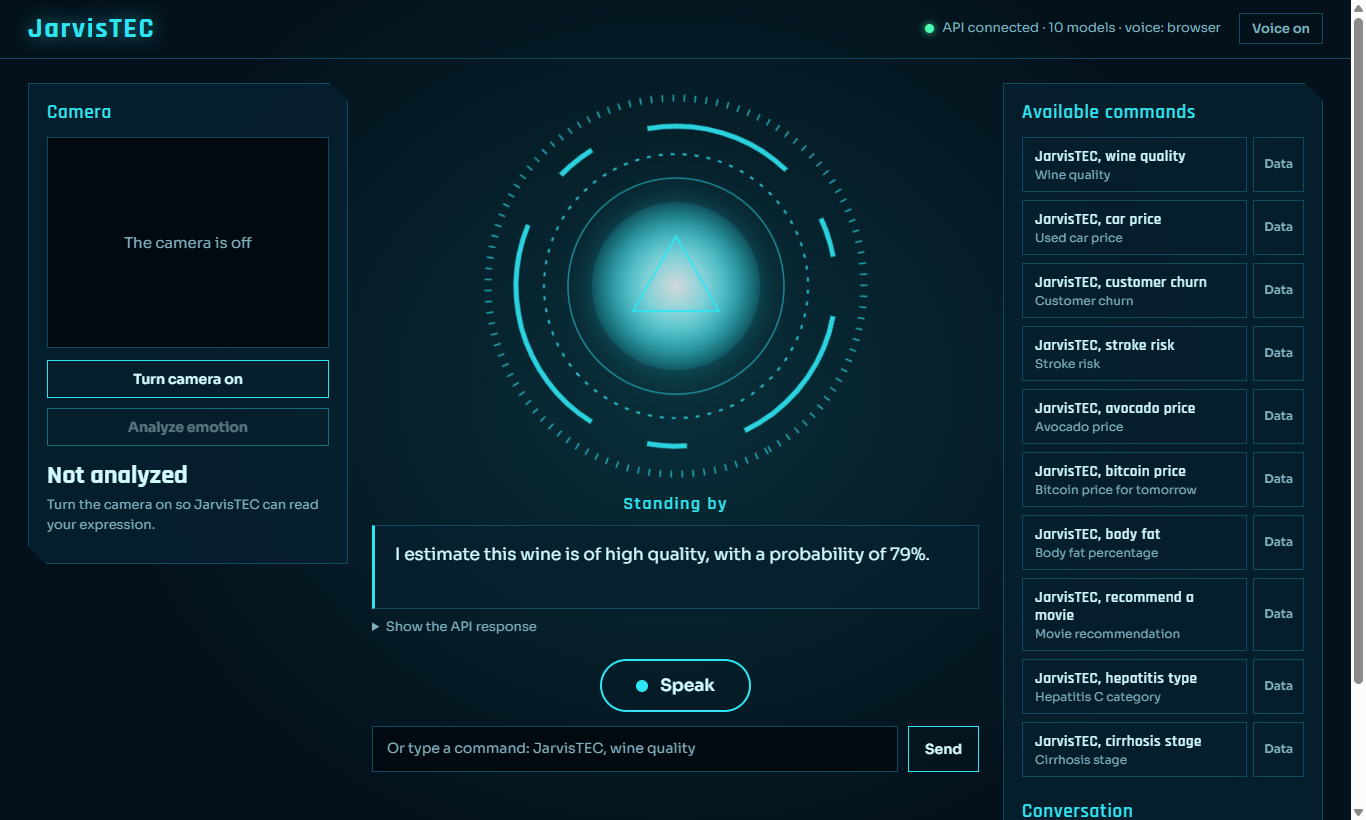
\includegraphics[width=\textwidth]{screenshot_interface.png}
\caption{The interface after the command ``JarvisTEC, wine quality'': camera panel, assistant answer and list of commands.}
\end{figure}

\begin{figure}[H]
\centering
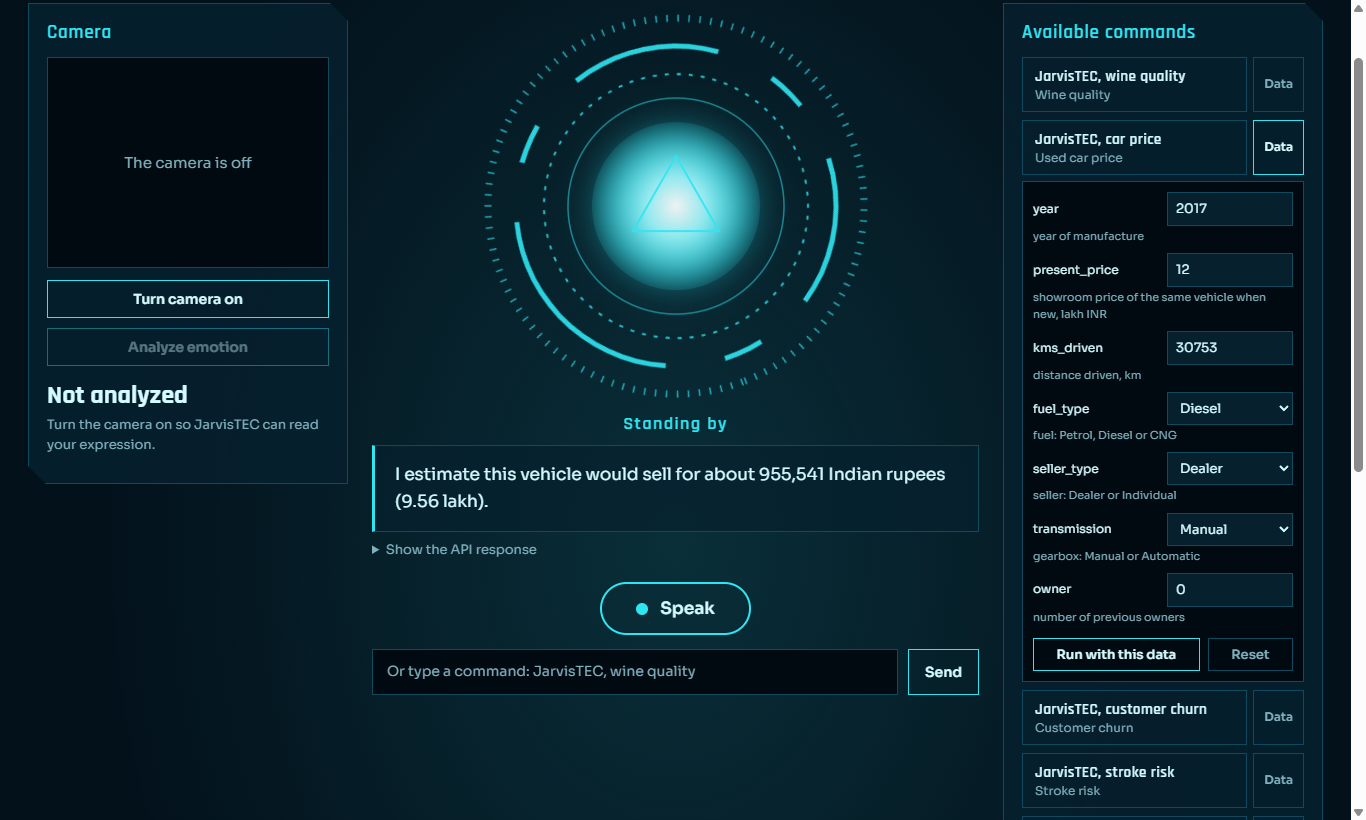
\includegraphics[width=\textwidth]{screenshot_data_form.png}
\caption{The data form of the car price model, generated from the model's input schema, and the answer for the edited values.}
\end{figure}

\begin{figure}[H]
\centering
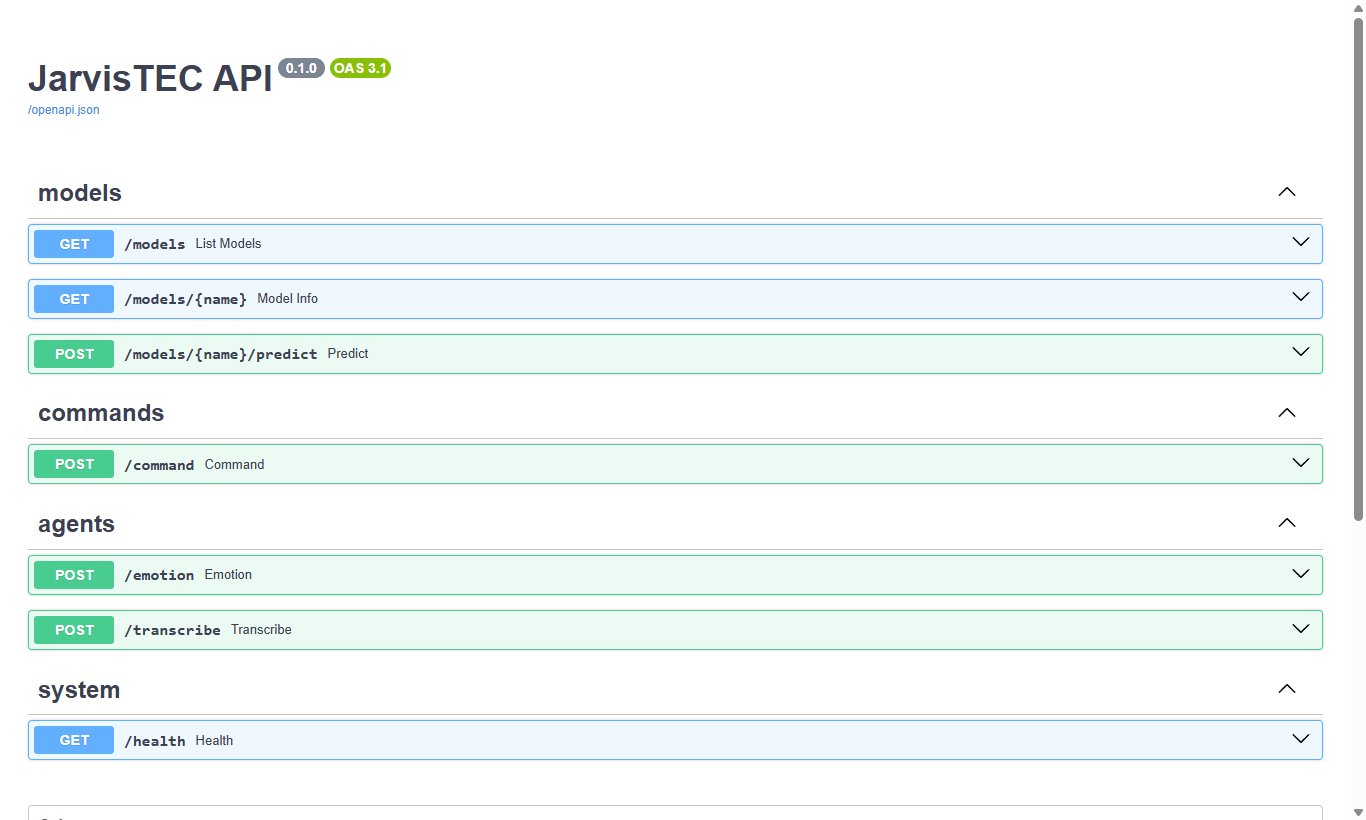
\includegraphics[width=0.9\textwidth]{screenshot_api_docs.png}
\caption{Interactive documentation of the REST API (\code{/docs}).}
\end{figure}

\end{document}
